\subsection{籽晶}
与有生命的动植物一样,培养优质单晶应选择优良的籽晶。籽晶上的缺陷,如位错、开裂、晶格畸变等在一定的范围内会“遗传”给新生长的晶体。避免使用有宏观缺陷的籽晶,有时还借助于物理光学的方法来挑选籽晶,以减少不利的“遗传”作用。

一般说来,结构和成分与结晶物质相同或相似的晶体取其中任何一部分都可以作为籽晶。但以结构和成分完全相同的完整晶体的一部分作籽晶时为最好。

同位素晶体:DKDP与KDP,DCDA与CDA,DTGS与TGS,DLAP与LAP等由于成分上只存在D与H的差异,结构上差异也不大,故可以互作为籽晶。钾明矾和铬矾的情况也相似。但是籽晶与新生长晶体在结构和成分上的差异会引起晶格失配,在晶体中留下应力,严重时会引起晶体开裂。所以籽晶最好取自相同生长条件下生长出来的完美晶体。

在初次培养一种新晶体时,可先培养出“晶芽”作为籽晶。对于溶解度正温度系数较大的结晶物质,培养“晶芽”是很方便的。先在烧杯中配制适量高于室温5---10摄氏度的饱和溶液,稍过热后注入5---10cm大的培养皿中,用表面皿盖好,让其在室温下冷却结晶,待七八小时后即可将尺寸较大、外形完美的“晶芽”用不锈钢镊子取出,用滤纸吸干溶液即成。如果“晶芽”尺寸不够大,可以把表面皿掀开一条缝,用控制蒸发的方法,让“晶芽”长到需要的尺寸。此法对溶解度温度系数小的结晶物质亦适用。

从已有的大晶体上切取籽晶是最方便和广泛使用的方法。根据晶体生长的习性和日后应用的要求,籽晶可采用“点”状,“杆”状或“片”状等不同的切型。一般来说,切割籽晶时应尽量保留在晶体生长慢的方向上有较大的尺寸。

KTN,$\rm NaNO_3$和NaCl一类晶体,各个方向生长速率相近,故可采用“点”状晶种。使用时将小粒晶种嵌入乳胶管一端,让完整性好的部分露出乳胶管,乳胶管的另一端套到掣晶杆上(图3.27)。“点”状籽晶生长过程恢复区很小,不利的“遗传”因素较易消除,晶体紧包住乳胶管生长,降低了掣晶杆与晶体间的应力。

\begin{figure}[htbp]
 \centering
 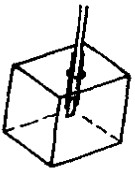
\includegraphics[width=0.4\textwidth]{fig/cp03/img3.27.jpg}
 \caption{点状籽晶($\rm NaNO_3$)。}
\end{figure}

\begin{figure}[htbp]
 \centering
 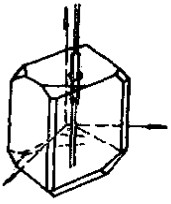
\includegraphics[width=0.4\textwidth]{fig/cp03/img3.28.jpg}
 \caption{杆状籽晶(TGS)。}
\end{figure}

TGS和LSH晶体$Z$向生长慢,采用平行于$Z$轴的“杆”状籽晶是合适的(图3.28)。由于在$X$,$Y$方向上生长较快,长出的晶体趋于各向匀称,这就提高了晶体产率和利用率。如采用平行于[111]晶稜的“杆”状籽晶来生产KDP型晶体,生长时恢复区很小,亦不需要成锥过程,对CDA,DCDA这类成锥较困难的晶体特别有意义(图3.29)。

实用上,生长KDP型晶体大都采用$Z$切片籽晶。这类晶体$Z$方向比$X$,$Y$方向生长快很多。$Z$切片籽晶在生长初期有一个恢复自然外形的成锥(俗称“成帽”)过程。生长成帽的地方主要在\{100\}和(001)相交的稜附近。保持籽晶在此稜附近的完整性对成帽质量起关键作用。籽晶片中央部分对生长影响较小,可以作打孔、捆绑或上螺丝将籽晶固定在掣晶架上。平行于KDP\{101\}切片也常用作籽晶,其好处是,平行于自然锥面,晶体生长恢复区小,降低了多个晶面生长引起的生长扇形界,后者使晶体光学均匀性变坏。此外,KDP晶体二类二倍频方向与\{101\}切片的方向接近,可以提高晶体的利用率。

ATGSAS采用平行于(010)的籽晶片,这样可以生长出单畴的大晶片,使整个晶片的均匀性大大提高,更适合于热成像技术上的应用。

晶体的生长习性是受生长条件影响的。所以实际工作中采用什么样的籽晶应同晶体生长习性,生长条件和应用要求结合起来考虑。

\begin{figure}[htbp]
 \centering
 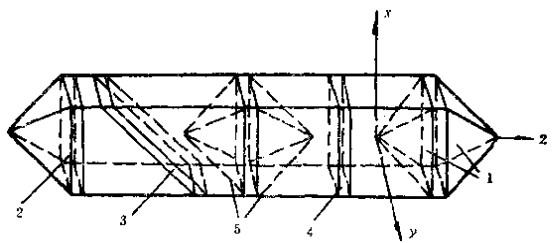
\includegraphics[width=0.8\textwidth]{fig/cp03/img3.29.jpg}
 \caption{KDP型晶体籽晶类型。图中:}
 1为全锥籽晶;2为半锥籽晶;3为平行锥面的\{011\}片状籽晶;
 4为$Z$切(001)片状籽晶;5为$Z$切片成锥。
\end{figure}